\documentclass[11pt,a4paper]{article}

\usepackage[utf8]{inputenc}
\usepackage[T1]{fontenc}
\usepackage{lmodern}
\usepackage[margin=2.2cm]{geometry}
\usepackage{amsmath}
\usepackage{booktabs}
\usepackage{xltabular}
\usepackage{array}
\usepackage{enumitem}
\usepackage[skip=8pt plus 2pt minus 1pt]{parskip} % space between paragraphs, no indent
\usepackage{xcolor}
\usepackage{tikz}
\usetikzlibrary{positioning,arrows.meta,fit,backgrounds,calc}
\usepackage{caption}
\usepackage[numbers,sort&compress]{natbib}
\usepackage[colorlinks=true,linkcolor=blue!50!black,urlcolor=blue!50!black,citecolor=blue!50!black]{hyperref}

\setlist{itemsep=2pt,topsep=4pt}
\renewcommand{\arraystretch}{1.25}
\newcolumntype{L}[1]{>{\raggedright\arraybackslash}p{#1}}
\newcolumntype{Y}{>{\raggedright\arraybackslash}X}

\definecolor{accent}{HTML}{2F6FDE}
\definecolor{band}{HTML}{F0EFEC}

\tikzset{
  box/.style={draw=black!45, rounded corners=4pt, align=center, font=\small,
              inner sep=5pt, minimum height=1.1cm},
  main/.style={box, draw=accent, line width=1.2pt, fill=accent!10},
  arr/.style={-{Stealth[length=2.2mm]}, draw=black!55, line width=0.7pt},
  note/.style={font=\footnotesize\color{black!60}},
}
\newcommand{\sub}[1]{{\footnotesize\color{black!60}#1}}

\title{Causal Inference Methods Guide:\\[2pt]
\large Measuring treatment effects from observational data\\[4pt]
\normalsize Target Trial Emulation, S-Learner, and Doubly Robust Causal Forest}
\author{Michael Allen\\ \href{mailto:m.allen@exeter.ac.uk}{\texttt{m.allen@exeter.ac.uk}}}
\date{\today}

\begin{document}
\maketitle
\begin{abstract}
\setlength{\parindent}{0pt}\setlength{\parskip}{6pt plus 2pt}% match body paragraph spacing
\noindent This guide is for analysts and clinicians who want to estimate the effect of a treatment from routinely collected (observational) data. It is not tied to one clinical area. In this guide, ``treatment'' can mean any intervention, drug, procedure or care pathway, and ``outcome'' any result of interest.

The guide describes three methods that work in different ways and answer the same question: among patients who received a treatment, how much did it change their chance of a good outcome?
\begin{enumerate}
\item \textbf{Target trial emulation with matching.} Each treated patient is compared with a similar untreated patient. This is transparent and easy to explain to clinicians. The guide covers both exact and non-exact matching, including propensity-score, Mahalanobis, full and risk-set matching.
\item \textbf{The S-learner.} A single prediction model is asked what would have happened to each patient with and without treatment. It can adjust for many confounders and for treatment timing.
\item \textbf{The doubly robust causal forest.} This uses double/debiased machine learning, which estimates individual treatment effects and stays reliable if either the treatment model or the outcome model is correct.
\end{enumerate}
For each method, the guide sets out how it works, the analysis steps, how to interpret the result, sensitivity analyses the authors have used, and further analyses that could be run.

Shared sections cover core concepts (the target trial framework, estimands such as the ATE, ATT and CATE, the assumptions every method needs, and choosing confounders); tools for assessing unmeasured and measured confounding (E-values, sensemakr robustness values, and leaving out one measured confounder at a time); a recommended workflow for choosing and combining the methods; and a plain-language glossary of more than 150 terms.

A final section briefly describes other methods, with their advantages and disadvantages, including the g-formula, TMLE, BART and designs that can allow for unmeasured confounding, such as instrumental variables and difference-in-differences.

The guide was developed in the SAMueL-3 project, alongside analyses of thrombolysis and thrombectomy in stroke using national audit data (SSNAP).

\medskip
\noindent\textbf{Keywords:} causal inference; target trial emulation; observational data; treatment effects; matching; propensity score; S-learner; meta-learners; causal forest; double machine learning; doubly robust estimation; sensitivity analysis; E-value; unmeasured confounding

\medskip
\noindent\textbf{How to cite this guide:} Allen, M. (2026). \emph{Causal Inference Methods Guide: Measuring treatment effects from observational data}. Zenodo. \href{https://doi.org/10.5281/zenodo.24426809}{doi:10.5281/zenodo.24426809} \cite{allen2026guide}.
\end{abstract}
\newpage
\tableofcontents
\newpage

% 01_overview.tex
\section{Overview}

This guide describes three complementary ways to estimate the effect of a treatment from routinely collected (observational) data, and the sensitivity analyses we use to test them. It is written to apply across clinical domains: wherever it says ``treatment'', read any intervention, drug, procedure or care pathway; wherever it says ``outcome'', read any patient outcome.

All three methods answer the same question: \emph{among patients who received the treatment, how much did it change their chance of the outcome?} They answer it in different ways, with different assumptions, so agreement between them is strong evidence, and disagreement points to where the data or assumptions are fragile.

\paragraph{A simple example.} Suppose 50\% of patients who received a treatment had a good outcome. The question is what that figure would have been if the \emph{same} patients had not been treated. If our best estimate is 40\%, the treatment added 10 percentage points: ten extra good outcomes for every 100 patients treated. All three methods estimate that missing 40\% figure. They differ only in how they build it from similar untreated patients.

\begin{xltabular}{\textwidth}{L{2.6cm}YYY}
\toprule
 & \textbf{Target trial emulation with exact matching} & \textbf{S-learner} & \textbf{Doubly robust causal forest} \\
\midrule
Core idea & Pair each treated patient with an identical untreated patient & One prediction model; ask it ``what if this patient had not been treated?'' & Remove the predictable part of treatment and outcome, then learn the effect from what is left \\
Adjusts for & A few key confounders, exactly & Many confounders, flexibly & Many confounders, flexibly, using two separate models (one predicting outcome, one predicting treatment) \\
Main strength & Transparent; easy to explain to clinicians & Handles continuous treatment timing and dose; flexible & If one of its two models is wrong, the other can compensate; can show who benefits most \\
Main weakness & Only a handful of confounders can be matched exactly & Relies entirely on one model being right; can shrink effects & Complex; individual effects are noisy \\
Typical software & pandas, statsmodels & XGBoost \cite{chen2016xgboost}, Optuna \cite{akiba2019optuna}, SHAP \cite{lundberg2017shap} & EconML \texttt{CausalForestDML} \cite{battocchi2019econml}, LightGBM \cite{ke2017lightgbm} \\
\bottomrule
\end{xltabular}

A \emph{confounder} is a factor, such as disease severity or frailty, that influences both whether a patient is treated and how they fare. No method can adjust for confounders that were not measured. Each method section therefore lists the sensitivity analyses that probe this, and the shared tools for unmeasured confounding are explained once, in Section~\ref{sec:shared}. Worked examples of all three methods, applied to stroke treatment, are in the SAMueL-3 repository \cite{samuel3}. Technical terms are defined in the glossary (Section~\ref{sec:glossary}).

% 02_core_concepts.tex
\section{Core concepts}

A treatment effect is the difference between what happened to a patient and what \emph{would} have happened to the same patient had their treatment been different. We only ever see one of these, so every method builds the missing one (the counterfactual) from similar patients \cite{hernan2020whatif}.

\subsection{The target trial}

Before any analysis, write down the randomised trial you would run if you could. This makes every design choice explicit and stops common errors such as comparing groups defined at different times. Use this protocol table at the start of every analysis \cite{hernan2016bigdata,hernan2025,cashin2025}. Aligning eligibility, treatment assignment and the start of follow-up at time zero prevents immortal-time and related selection biases \cite{hernan2016immortal}.

\begin{xltabular}{\textwidth}{L{4cm}Y}
\toprule
\textbf{Component} & \textbf{What to specify} \\
\midrule
Eligibility & Who could have received either treatment at time zero \\
Treatment strategies & The treatment(s), including timing or dose, and the comparator (often ``no treatment'') \\
Assignment & In a trial, random. In observational data, replaced by adjustment for confounders \\
Time zero & When eligibility is met and follow-up starts. It must be the same for both arms \\
Follow-up and outcome & What is measured, and when \\
Causal contrast & Which estimand (below) \\
Analysis & How the contrast is estimated, and how uncertainty is quantified \\
\bottomrule
\end{xltabular}

\subsection{Estimands: what exactly are we estimating?}

An \emph{estimand} is the precise quantity an analysis sets out to estimate: which effect, in which patients, on which scale. Stating it up front makes clear what question the result answers. The three estimands used in this guide are:

\begin{xltabular}{\textwidth}{L{3.2cm}YY}
\toprule
\textbf{Estimand} & \textbf{Question it answers} & \textbf{When to prefer it} \\
\midrule
ATT: average effect in the treated & How much did treatment help the patients who actually received it? & Evaluating current practice; needs comparable untreated patients for each treated patient only \\
ATE: average effect in everyone & What if everyone eligible were treated? & Policy questions about extending treatment; needs every type of patient to have some chance of treatment \\
CATE: conditional effect & How does the effect vary with patient characteristics? & Targeting treatment; individual estimates are noisy and need validating \\
\bottomrule
\end{xltabular}

Our default is the \textbf{ATT}, reported as an absolute difference in the probability of the outcome (percentage points), with a relative effect (risk ratio) alongside. In clinical terms, the ATT asks ``did treatment help the patients we chose to treat?'', whereas the ATE asks ``what would happen if we treated everyone eligible?''.

\subsection{Assumptions every method needs}

\begin{xltabular}{\textwidth}{L{3.4cm}YY}
\toprule
\textbf{Assumption} & \textbf{Plain meaning} & \textbf{How we check it} \\
\midrule
No unmeasured confounding (exchangeability) & Once we account for the measured variables, treated and untreated patients are comparable & Cannot be proven; probed with E-values \cite{vanderweele2017evalue}, sensemakr \cite{cinelli2020} and leave-one-out \\
Positivity (overlap) & Each type of treated patient has comparable untreated patients & Percentage matched; propensity score distributions \cite{rosenbaum1983}; trimming \cite{crump2009} \\
Consistency & ``Treatment'' means the same thing for everyone in a group & Define strategies precisely (e.g.\ by timing or dose); vary definitions \\
No interference & One patient's treatment does not change another's outcome & Usually assumed in individual-level clinical data \\
Correct timing & Covariates are measured before treatment; time zero is the same in both arms & Design review; landmark analyses \cite{hernan2016immortal} \\
\bottomrule
\end{xltabular}

In practice the first assumption is the weakest. Clinicians often decide on treatment using information that is never recorded, such as how unwell a patient looks, their wishes or imaging findings. If that information also predicts outcome, every method will be biased. This is why each method section includes sensitivity analyses for unmeasured confounding.

\subsection{Choosing confounders}

Adjust for variables that affect both treatment and outcome and are measured before treatment. Do \textbf{not} adjust for variables on the pathway from treatment to outcome (mediators), or for variables that only determine treatment timing when timing is part of the strategy, because that removes part of the effect being estimated. Draw a directed acyclic graph (DAG) to decide each variable's role \cite{hernan2020whatif}, and test borderline variables as sensitivity analyses.

% 03_target_trial_emulation.tex
\section{Method 1: Target trial emulation with exact matching}

\subsection{How it works}

For each treated patient, we find an untreated patient who is identical on the most important confounders, such as age, disease severity and prior disability. We then compare outcomes between the two matched groups. Because each pair looks alike on the factors that drive both treatment and outcome, the untreated partner stands in for what would have happened to the treated patient without treatment.

It is the observational equivalent of a randomised trial in which randomisation is replaced by matching \cite{hernan2016bigdata,stuart2010}. Its strength is transparency: a clinician can see exactly who is compared with whom, and check that the groups look alike.

\begin{figure}[!htbp]
\centering
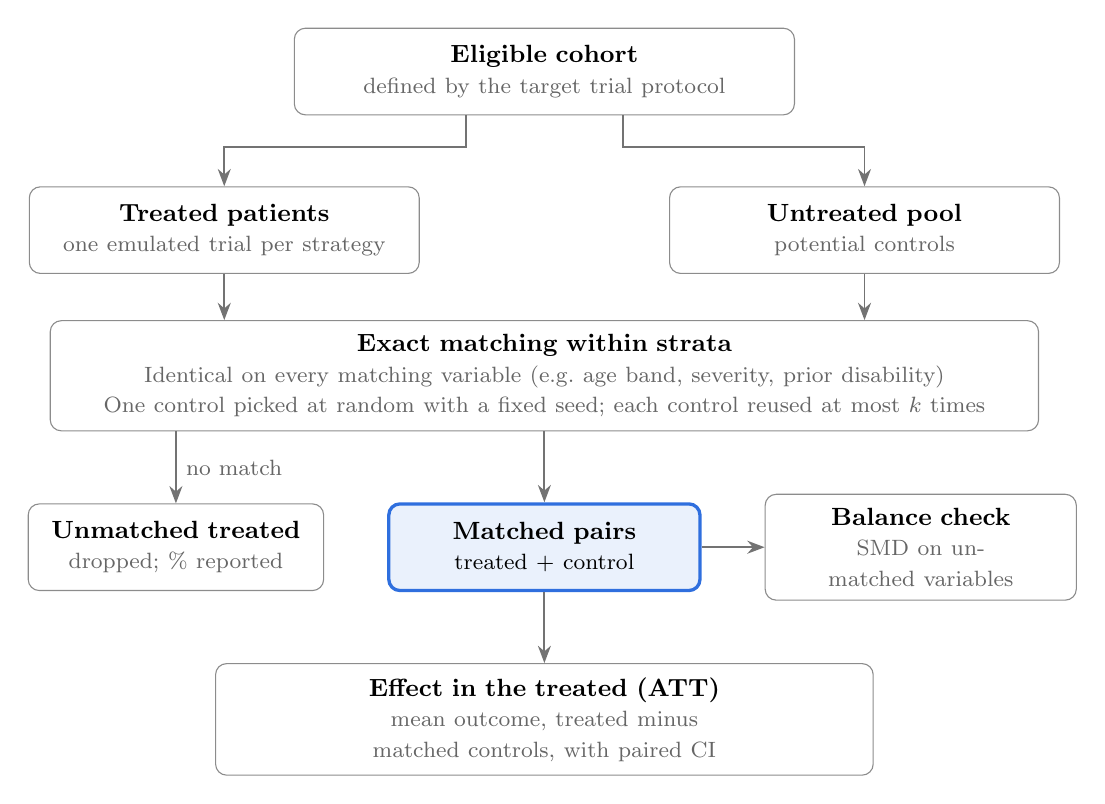
\begin{tikzpicture}[node distance=0.75cm]
\node[box, text width=6cm] (cohort) {\textbf{Eligible cohort}\\ \sub{defined by the target trial protocol}};
\node[box, text width=4.6cm, below left=0.9cm and -1.6cm of cohort] (treated) {\textbf{Treated patients}\\ \sub{one emulated trial per strategy}};
\node[box, text width=4.6cm, below right=0.9cm and -1.6cm of cohort] (untreated) {\textbf{Untreated pool}\\ \sub{potential controls}};
\node[box, text width=12.2cm, below=2.6cm of cohort] (match) {\textbf{Exact matching within strata}\\ \sub{Identical on every matching variable (e.g.\ age band, severity, prior disability)}\\ \sub{One control picked at random with a fixed seed; each control reused at most $k$ times}};
\node[main, text width=3.6cm, below=0.9cm of match] (pairs) {\textbf{Matched pairs}\\ \footnotesize treated + control};
\node[box, text width=3.4cm, left=0.8cm of pairs] (unmatched) {\textbf{Unmatched treated}\\ \sub{dropped; \% reported}};
\node[box, text width=3.6cm, right=0.8cm of pairs] (balance) {\textbf{Balance check}\\ \sub{SMD on unmatched variables}};
\node[box, text width=8cm, below=0.9cm of pairs] (att) {\textbf{Effect in the treated (ATT)}\\ \sub{mean outcome, treated minus matched controls, with paired CI}};
\draw[arr] (cohort.south) ++(-1,0) |- ++(0,-0.4) -| (treated.north);
\draw[arr] (cohort.south) ++(1,0) |- ++(0,-0.4) -| (untreated.north);
\draw[arr] (treated.south) -- (treated.south |- match.north);
\draw[arr] (untreated.south) -- (untreated.south |- match.north);
\draw[arr] (match.south) -- (pairs.north);
\draw[arr] (unmatched.north |- match.south) -- node[right, note] {no match} (unmatched.north);
\draw[arr] (pairs.east) -- (balance.west);
\draw[arr] (pairs.south) -- (att.north);
\end{tikzpicture}
\caption{Exact matching workflow. Treated patients without an identical untreated partner are dropped, so the matching rate shows how far the result represents all treated patients.}
\label{fig:matching}
\end{figure}

\subsection{Steps}

\begin{enumerate}
\item \textbf{Define the cohort and strategies} using the target trial protocol. Each treatment strategy (e.g.\ early vs late, drug A vs none) gets its own emulated trial with its own matched controls.
\item \textbf{Choose matching variables:} a small number (typically 4--6) of strong, pre-treatment confounders. Continuous variables are banded (e.g.\ 5-year age bands) so that exact matches exist.
\item \textbf{Match exactly.} Within each stratum of identical values, pick an untreated control at random with a fixed seed. Decide whether a control may be reused (e.g.\ up to 3 times) or not (1:1 without replacement); reuse raises the matching rate but makes pairs less independent.
\item \textbf{Report the matching rate} (percentage of treated patients matched). A low rate means the result applies to a subset of treated patients.
\item \textbf{Check balance} on variables that were \emph{not} matched, using standardised mean differences (SMD); an absolute SMD below 0.1 is usually taken as good balance \cite{austin2009}. In words, the SMD is how far apart the two groups' averages are, measured in standard deviations, so it can be compared across variables measured in different units:
\[ \mathrm{SMD} = \frac{\bar{x}_T - \bar{x}_C}{\sqrt{(s_T^2 + s_C^2)/2}} \]
\item \textbf{Estimate the effect:} difference in outcome proportions (or means) between matched treated and matched controls, with a paired analysis that respects the matching (McNemar's test, paired $t$ or Wilcoxon), or cluster-robust confidence intervals when one control is matched to several treated patients. Adjust for multiplicity (e.g.\ Holm \cite{holm1979}) when many trials are run.
\end{enumerate}

\subsection{What the result means}

The estimate is the ATT. Each strategy is compared with its own controls, so effects for different strategies describe different kinds of patients and are not a head-to-head comparison.

\subsection{Sensitivity analyses we have used}

\begin{xltabular}{\textwidth}{L{2.6cm}YY}
\toprule
\textbf{Group} & \textbf{Analysis} & \textbf{What it tests} \\
\midrule
\endhead
Inference & Paired or cluster-robust CIs (cluster on control) & Pairs that share a reused control are not independent \\
Randomness & Repeat matching with 20 random seeds; report median, min, max & Dependence on which control was picked at random \\
Matching design & Control reuse: once, up to 3, up to 5, unlimited & Trade-off between matching rate and independence \\
Matching design & Reverse the order in which strategies are matched & Order effects when the reuse limit is shared \\
Matching design & Finer matching (e.g.\ exact score instead of band) & Residual confounding within bands \\
Matching design & Add further confounders (e.g.\ comorbidities, sex) & Confounding by variables only checked for balance \\
Matching design & Restrict or match on a key clinical marker recorded for only some patients & Confounding by a strong but incompletely recorded variable \\
Cohort & Restrict to patients with complete timing data & Misclassification of treatment timing \\
Cohort & Vary site-volume or provider restrictions & Whether results depend on which centres are included \\
Cohort & Include or exclude subgroups selected by special investigations & Selection by indication \\
Cohort & Narrower eligibility windows & Whether untreated patients had a real chance of treatment \\
Treatment definition & Vary the early/late (or dose) cut-off & Choice of threshold \\
Time & Landmark analysis (keep only pairs alive and in follow-up at a fixed time) & Immortal-time bias \cite{hernan2016immortal} \\
Outcome & Stricter and looser outcome definitions; secondary outcomes (death, length of stay, destination) & Dependence on outcome definition; consistency across outcomes \\
Outcome & Length of stay in survivors only & Separating effects on recovery from effects on survival \\
Unmeasured confounding & E-values \cite{vanderweele2017evalue}; sensemakr \cite{cinelli2020} on a linear model in the matched sample & How strong a hidden confounder would need to be \\
Measured confounding & Leave each main matching variable out in turn & How much the result depends on each confounder \\
\bottomrule
\end{xltabular}

\subsection{Further analyses that could be run}

\begin{itemize}
\item \textbf{Coarsened exact \cite{iacus2012} or propensity-score matching \cite{rosenbaum1983,stuart2010}} to include more confounders while keeping most treated patients; compare with exact matching.
\item \textbf{Regression adjustment within matched pairs} (doubly robust matching) to remove residual imbalance in unmatched variables.
\item \textbf{Clone-censor-weight designs} \cite{hernan2018duration} for strategies defined by timing, which handle immortal time properly rather than by landmark.
\item \textbf{Averaging over many matchings} (or reporting the median across seeds) as the primary estimate, so that the result does not depend on one random draw.
\item \textbf{Negative-control outcomes} (outcomes the treatment cannot affect) to detect residual confounding \cite{lipsitch2010}.
\item \textbf{Calibration against trial results} in the subgroup that most resembles a randomised trial population.
\end{itemize}

% 04_s_learner.tex
\section{Method 2: S-learner}

\subsection{How it works}

We train one machine-learning model (the ``single learner'' \cite{kunzel2019}) to predict each patient's outcome from their characteristics \emph{and} the treatment they received. Once the model has learned how outcomes depend on both, we ask it a ``what if'' question for each treated patient: \emph{what would this patient's predicted outcome be if they had not been treated?} The difference between the two predictions is that patient's estimated benefit. Averaging over treated patients gives the ATT.

A useful way to think of it is as a very detailed risk calculator that includes treatment as one of its inputs. We enter each treated patient's details twice, once with their treatment and once with treatment switched off, and read off the difference in predicted risk.

Because treatment is just another input, the model can represent treatment as a continuous quantity, such as time to treatment or dose. This makes the S-learner the natural tool for questions like ``how quickly does benefit fall with delay?''

\begin{figure}[!htbp]
\centering
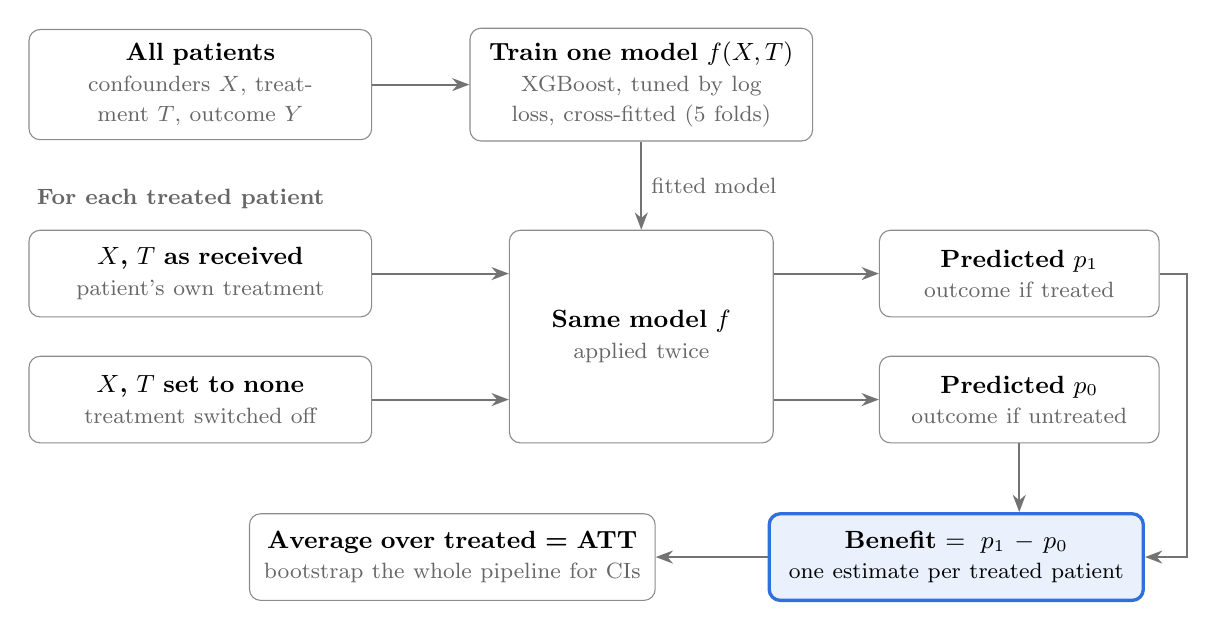
\begin{tikzpicture}
\node[box, text width=4cm] (data) at (0,0) {\textbf{All patients}\\ \sub{confounders $X$, treatment $T$, outcome $Y$}};
\node[box, text width=4cm] (train) at (5.6,0) {\textbf{Train one model $f(X,T)$}\\ \sub{XGBoost, tuned by log loss, cross-fitted (5 folds)}};
\node[font=\footnotesize\bfseries\color{black!60}, anchor=west] at (-2.2,-1.45) {For each treated patient};
\node[box, text width=4cm] (in1) at (0,-2.4) {\textbf{$X$, $T$ as received}\\ \sub{patient's own treatment}};
\node[box, text width=4cm] (in0) at (0,-4.0) {\textbf{$X$, $T$ set to none}\\ \sub{treatment switched off}};
\node[box, text width=3cm, minimum height=2.7cm] (model) at (5.6,-3.2) {\textbf{Same model $f$}\\ \sub{applied twice}};
\node[box, text width=3.2cm] (p1) at (10.4,-2.4) {\textbf{Predicted $p_1$}\\ \sub{outcome if treated}};
\node[box, text width=3.2cm] (p0) at (10.4,-4.0) {\textbf{Predicted $p_0$}\\ \sub{outcome if untreated}};
\node[main, text width=4.4cm] (ben) at (9.6,-6.0) {\textbf{Benefit $= p_1 - p_0$}\\ \footnotesize one estimate per treated patient};
\node[box, text width=4.8cm] (att) at (3.2,-6.0) {\textbf{Average over treated = ATT}\\ \sub{bootstrap the whole pipeline for CIs}};
\draw[arr] (data) -- (train);
\draw[arr] (train) -- node[right, note] {fitted model} (model);
\draw[arr] (in1.east) -- (in1.east -| model.west);
\draw[arr] (in0.east) -- (in0.east -| model.west);
\draw[arr] (p1.west -| model.east) -- (p1.west);
\draw[arr] (p0.west -| model.east) -- (p0.west);
\draw[arr] (p0.south) -- (p0.south |- ben.north);
\draw[arr] (p1.east) -- ++(0.35,0) |- (ben.east);
\draw[arr] (ben.west) -- (att.east);
\end{tikzpicture}
\caption{S-learner counterfactual prediction. The only thing that changes between the two predictions is the treatment input, so their difference is the model's estimate of what treatment did for that patient.}
\label{fig:slearner}
\end{figure}

\subsection{Steps}

\begin{enumerate}
\item \textbf{Features:} all measured pre-treatment confounders, plus treatment. Treatment can be a category (e.g.\ strategy arms) or continuous (e.g.\ time to treatment, with a sentinel value far outside the real range meaning ``not given'').
\item \textbf{Model:} gradient-boosted trees (XGBoost \cite{chen2016xgboost}), which capture non-linear effects and interactions. Categorical variables such as site can be handled natively.
\item \textbf{Tuning:} choose hyperparameters by cross-validated \textbf{log loss} (e.g.\ with Optuna \cite{akiba2019optuna}), not accuracy or AUC, because log loss penalises over-confident wrong predictions and so rewards probabilities that match reality. Do not use class weighting (artificially up-weighting the rarer outcome): it pushes predicted probabilities away from the true risks.
\item \textbf{Cross-fitting:} split patients into folds (e.g.\ 5). Each fold is predicted by a model trained on the others, so no patient's prediction comes from a model that saw them.
\item \textbf{Counterfactual prediction:} for each treated patient, predict with treatment as received and with treatment set to ``none''. Benefit = difference, on the probability scale (percentage points) and log-odds scale.
\item \textbf{Summarise:} mean benefit per treatment group (ATT); benefit against continuous treatment (e.g.\ regression of benefit on time, giving the slope and the time at which benefit reaches zero). With intercept $a$ and slope $b$, the zero point and its delta-method variance are
\[ x_0 = -\frac{a}{b}, \qquad \mathrm{Var}(x_0) = \frac{\mathrm{Var}(a)}{b^2} + \frac{a^2\,\mathrm{Var}(b)}{b^4} - \frac{2a\,\mathrm{Cov}(a,b)}{b^3}. \]
In words: fit a straight line of predicted benefit against delay; where the line crosses zero is the delay beyond which the model predicts no benefit. If that point lies beyond the treatment times actually seen in the data, it is an extrapolation and should be reported as such.
\item \textbf{Uncertainty:} bootstrap the whole pipeline (refit on resampled data). Confidence intervals from the spread of individual benefits are far too narrow and must not be reported as uncertainty.
\item \textbf{Heterogeneity:} fit a ``meta-model'' to the individual benefits and explain it with SHAP \cite{lundberg2017shap}, which shows how much each patient characteristic pushes predicted benefit up or down, to describe who benefits more or less.
\end{enumerate}

\subsection{What the result means}

The estimate is only as good as the outcome model. Check discrimination (out-of-fold AUC: how well the model ranks patients by risk) and, more importantly, calibration (whether a predicted 30\% chance really corresponds to about 30\% of such patients having the outcome; summarised by a calibration slope near 1, intercept near 0, and deciles close to the diagonal), because effects are differences between predicted probabilities \cite{vancalster2019}. Report both following TRIPOD \cite{collins2015tripod}. The meta-model only describes the S-learner's own estimates; it cannot find variation the S-learner missed.

A known weakness: if the model gives little weight to the treatment feature (for example, under heavy regularisation), estimated effects shrink towards zero \cite{kunzel2019}.

\subsection{Sensitivity analyses we have used}

\begin{xltabular}{\textwidth}{L{2.6cm}YY}
\toprule
\textbf{Group} & \textbf{Analysis} & \textbf{What it tests} \\
\midrule
\endhead
Overlap & Propensity model for treatment; distribution by arm; \% outside 0.05--0.95 & Whether treated patients have comparable untreated patients \\
Overlap & Re-estimate after trimming propensities outside 0.05--0.95 \cite{crump2009} & Dependence on extrapolation \\
Randomness & Different cross-validation seeds & Dependence on fold allocation \\
Uncertainty & Bootstrap of the whole pipeline & Model uncertainty \\
Model specification & Default (untuned) settings, with and without class weighting & Effect of tuning and of class weighting on calibration and effect size \\
Model specification & Fixed, heavily regularised model & Model flexibility \\
Model specification & Logistic regression S-learner (main effects) & Model class; no interactions \\
Confounder set & Without site / provider & Reliance on adjusting for local practice \\
Treatment definition & Vary early/late or dose cut-offs & Choice of threshold \\
Cohort & Restrict to more severe patients; narrower eligibility windows; previously independent patients only & Dependence on population \\
Outcome & Stricter and looser definitions & Dependence on outcome definition \\
Unmeasured confounding & E-values \cite{vanderweele2017evalue} (with $RR \approx \sqrt{OR}$ for common outcomes \cite{vanderweele2017sqrt}) & How strong a hidden confounder would need to be \\
Unmeasured confounding & Sensemakr \cite{cinelli2020} on a linear probability model (arm vs all untreated) & Same, on the explained-variance scale, with measured benchmarks \\
Measured confounding & Leave each main confounder out in turn and refit & How much the result depends on each confounder \\
\bottomrule
\end{xltabular}

\subsection{Further analyses that could be run}

\begin{itemize}
\item \textbf{Other meta-learners:} T-learner (separate treated and untreated models), X-learner \cite{kunzel2019} and DR-learner \cite{kennedy2023}, which avoid the S-learner's shrinkage towards zero.
\item \textbf{Nested tuning} (re-tuning inside each training fold) to remove the small optimism from tuning on all patients.
\item \textbf{Placebo tests:} randomly reassign treatment times among treated patients; any time gradient should disappear.
\item \textbf{Negative-control outcomes} that the treatment cannot affect but share confounders \cite{lipsitch2010}.
\item \textbf{Instrumental variable analysis} using between-site variation in treatment rates, which under its own assumptions addresses unmeasured patient-level confounding \cite{baiocchi2014}.
\item \textbf{Quantitative bias analysis} for a named unmeasured confounder, using plausible prevalences and effect sizes \cite{lash2014}.
\item \textbf{Multiple imputation} of missing covariates, compared with the model's native handling of missing values.
\item \textbf{Comparison with trial evidence} in the subgroup most like a trial population.
\end{itemize}

% 05_causal_forest.tex
\section{Method 3: Doubly robust causal forest}

\subsection{How it works}

The method asks: \emph{for patients who look alike, did those who were treated do better than we would have expected?} It works in two stages \cite{chernozhukov2018,wager2018,athey2019}.

In the \textbf{first stage}, two prediction models are built. One predicts each patient's outcome from their characteristics, ignoring treatment. The other predicts each patient's probability of receiving each treatment (the propensity score). Subtracting these predictions from what actually happened leaves two residuals: how much better or worse the outcome was than expected, and how far the treatment differed from what is typical for similar patients. Removing the predictable part of both is how the method adjusts for confounding, including confounding by indication.

In the \textbf{second stage}, a causal forest relates the outcome residuals to the treatment residuals \cite{nie2021,athey2019}, splitting patients into subgroups where the effect differs. As an illustration, a patient predicted to have a 30\% chance of a good outcome who then has one has a large, positive outcome residual. A patient predicted to have a 90\% chance of being treated who is treated has a small treatment residual, because their treatment was unsurprising. The method therefore learns mainly from patients whose treatment was \emph{not} predictable from their characteristics: patients who could reasonably have gone either way, which is where treated and untreated patients are most alike.

The forest gives an estimated effect for every patient (the conditional effect, CATE). The headline estimate then combines both first-stage models in a \textbf{doubly robust} (augmented inverse-probability-weighted, AIPW \cite{robins1994}) average, which is correct if \emph{either} the outcome model or the propensity model is correct, and is only weakly affected by small errors in either. Put simply, because it uses both models, a mistake in one can be compensated by the other.

\begin{figure}[!htbp]
\centering
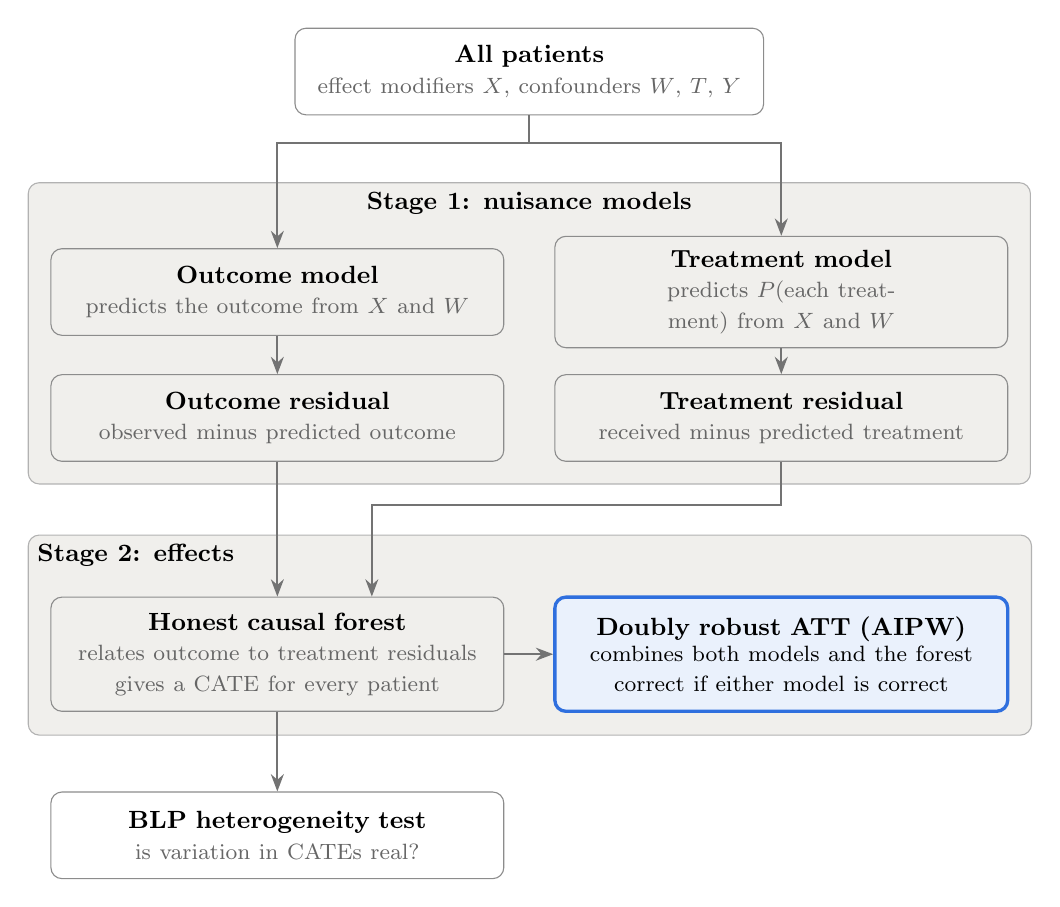
\begin{tikzpicture}
\node[box, text width=5.6cm] (data) at (0,0.7) {\textbf{All patients}\\ \sub{effect modifiers $X$, confounders $W$, $T$, $Y$}};
\node[box, text width=5.4cm] (om) at (-3.2,-2.1) {\textbf{Outcome model}\\ \sub{predicts the outcome from $X$ and $W$}};
\node[box, text width=5.4cm] (tm) at (3.2,-2.1) {\textbf{Treatment model}\\ \sub{predicts $P$(each treatment) from $X$ and $W$}};
\node[box, text width=5.4cm] (or) at (-3.2,-3.7) {\textbf{Outcome residual}\\ \sub{observed minus predicted outcome}};
\node[box, text width=5.4cm] (tr) at (3.2,-3.7) {\textbf{Treatment residual}\\ \sub{received minus predicted treatment}};
\node[box, text width=5.4cm, minimum height=1.45cm] (forest) at (-3.2,-6.7) {\textbf{Honest causal forest}\\ \sub{relates outcome to treatment residuals}\\ \sub{gives a CATE for every patient}};
\node[main, text width=5.4cm, minimum height=1.45cm] (aipw) at (3.2,-6.7) {\textbf{Doubly robust ATT (AIPW)}\\ \footnotesize combines both models and the forest\\ \footnotesize correct if either model is correct};
\node[box, text width=5.4cm] (blp) at (-3.2,-9.0) {\textbf{BLP heterogeneity test}\\ \sub{is variation in CATEs real?}};
\coordinate (s1top) at ($(om.north)+(0,0.55)$);
\coordinate (s2top) at ($(forest.north)+(0,0.5)$);
\begin{scope}[on background layer]
\node[fill=band, draw=black!30, rounded corners=4pt, inner sep=8pt, fit=(om) (tm) (or) (tr) (s1top), label={[anchor=north, font=\small\bfseries]north:Stage 1: nuisance models}] (s1) {};
\node[fill=band, draw=black!30, rounded corners=4pt, inner sep=8pt, fit=(forest) (aipw) (s2top), label={[anchor=north west, font=\small\bfseries]north west:Stage 2: effects}] (s2) {};
\end{scope}
\draw[arr] (data.south) -- ++(0,-0.35) -| (om.north);
\draw[arr] (data.south) -- ++(0,-0.35) -| (tm.north);
\draw[arr] (om) -- (or);
\draw[arr] (tm) -- (tr);
\draw[arr] (or.south) -- (forest.north);
\draw[arr] (tr.south) -- ++(0,-0.55) -| ($(forest.north)+(1.2,0)$);
\draw[arr] (forest) -- (aipw);
\draw[arr] (forest.south) -- (blp.north);
\end{tikzpicture}
\caption{Two-stage doubly robust causal forest. Stage 1 strips out what can be predicted from patient characteristics; Stage 2 learns the effect from what is left and combines both first-stage models into the headline ATT.}
\label{fig:forest}
\end{figure}

\subsection{Steps}

\begin{enumerate}
\item \textbf{Split variables into two roles.} $X$ are effect modifiers the forest may split on (clinical characteristics). $W$ are additional confounders used only in the first stage (e.g.\ site, calendar year). $X$ is always included in the first stage too. In practice, clinical features go in $X$, and administrative or practice factors such as hospital or year go in $W$.
\item \textbf{First stage (nuisance models):} gradient-boosted trees (LightGBM \cite{ke2017lightgbm}) for the outcome and for a multiclass treatment model, with cross-fitting (e.g.\ 5 folds) so each patient's predictions come from models trained on others.
\item \textbf{Second stage:} an honest causal forest (e.g.\ 2,000 trees, minimum leaf size around 25). ``Honest'' means each tree uses half its sample to choose splits and the other half to estimate effects, reducing overfitting \cite{athey2016,wager2018}. We use EconML \texttt{CausalForestDML} \cite{battocchi2019econml}.
\item \textbf{ATT by AIPW:} the ATT (average treatment effect in the treated) is the average effect of treatment among the patients who actually received it. AIPW (augmented inverse-probability weighting) is a doubly robust way to estimate it, combining the outcome model with propensity-score weights, so the estimate is correct if either model is correct. For each treated patient, we estimate what would have happened without treatment by combining the outcome model's prediction with a correction based on similar untreated patients. Each untreated patient is weighted by $P(\text{treatment}) / P(\text{no treatment})$, so those who most resemble treated patients count for more. Very small probabilities are capped (``clipped'', e.g.\ at 0.01) so that no single patient receives an enormous weight. Confidence intervals come from the influence function, a standard formula for this estimator. Avoid unclipped built-in estimators: tiny propensities give enormous weights and implausible results.
\item \textbf{Other estimates:} report the ATE only where overlap is good across the whole cohort (e.g.\ fewer than 20\% of patients below the clip). Also report the risk ratio in the treated, and the mean CATE among treated patients (without a CI, because the individual estimates share trees and are not independent).
\item \textbf{Heterogeneity:} the best linear predictor (BLP) test \cite{chernozhukov2025} regresses the doubly robust effect on the forest's out-of-bag CATE. A slope above 0 means real variation in benefit is detected; near 1 means the individual estimates are well calibrated. In plain terms, it checks whether patients the forest predicts will benefit more really do benefit more. If the slope is weak, report subgroup ATTs with a test of equal effects, not individual CATEs.
\end{enumerate}

\subsection{What the result means}

The AIPW ATT is the most reliable estimate from this method. Individual CATEs are noisy; use them to describe patterns, not to make decisions about individual patients, unless the BLP test supports it. Check first-stage discrimination and calibration, and overlap (the share of treated patients with very low probability of no treatment).

\subsection{Sensitivity analyses we have used}

\begin{xltabular}{\textwidth}{L{2.6cm}YY}
\toprule
\textbf{Group} & \textbf{Analysis} & \textbf{What it tests} \\
\midrule
\endhead
Overlap & Distribution of $P$(no treatment) among treated; \% below 0.05 and 0.01 \cite{crump2009} & Whether comparable untreated patients exist \\
Overlap & Exclude patients with $P$(no treatment) $< 0.05$ & Dependence on extreme weights \\
Randomness & Several random seeds & Cross-fitting splits, subsampling, forest randomness \\
Model specification & Smaller first-stage models & First-stage complexity \\
Model specification & Larger minimum leaf size & Forest settings \\
Model specification & Alternative categorical encoding of $X$ and $W$ & Encoding errors \\
Cross-fitting & Folds grouped by site & Whether predictions generalise to unseen sites \\
Confounder set & Without site & Reliance on adjusting for local practice \\
Confounder set & Add timing variables (e.g.\ time to first assessment) and calendar year & Whether a variable that drives treatment timing should be adjusted for \\
Confounder set & Add an incompletely recorded clinical marker (missing as its own category) & Confounding by a strong but partly recorded variable \\
Treatment definition & Vary early/late or dose cut-offs & Choice of threshold \\
Cohort & Narrower eligibility windows; vary site-volume restriction & Dependence on population \\
Outcome & Stricter and looser definitions & Dependence on outcome definition \\
Cross-method & Compare subgroup ATTs with the matched target trial emulation & Agreement across different assumptions \\
Unmeasured confounding & E-values (RR from observed treated proportion $p_1$ and $p_1 - \mathrm{ATT}$) \cite{vanderweele2017evalue}; sensemakr \cite{cinelli2020} on a linear model with the same confounders & How strong a hidden confounder would need to be \\
Measured confounding & Leave each main confounder out in turn and refit & How much the result depends on each confounder \\
\bottomrule
\end{xltabular}

\subsection{Further analyses that could be run}

\begin{itemize}
\item \textbf{Policy learning:} use the CATEs to derive and evaluate a simple treatment rule (e.g.\ a shallow policy tree), with honest out-of-sample evaluation \cite{athey2021}.
\item \textbf{Calibration of CATEs} by quantile groups (group average treatment effects, GATES) and classification analysis (CLAN) to describe who benefits most \cite{chernozhukov2025}.
\item \textbf{Alternative doubly robust estimators} (DR-learner \cite{kennedy2023}, targeted maximum likelihood estimation \cite{vanderlaan2006}) for comparison.
\item \textbf{Continuous treatment} (e.g.\ time or dose) using a continuous-treatment DML model \cite{chernozhukov2018}, rather than fixed categories.
\item \textbf{Instrumental-variable forest} using between-site variation \cite{athey2019,baiocchi2014}, to address unmeasured patient-level confounding.
\item \textbf{Negative-control outcomes and exposures} \cite{lipsitch2010}.
\item \textbf{Transportability:} re-weight the ATT to a target population (e.g.\ a trial population or another region) \cite{dahabreh2019}.
\end{itemize}

% 06_confounding_tools.tex
\section{Shared tools for confounding}\label{sec:shared}

Three tools are applied with every method. E-values and sensemakr ask \emph{how strong would a hidden confounder need to be?} Leave-one-out asks \emph{how much does the result actually depend on the confounders we have?} In our experience leave-one-out is often the most revealing, because it shows which single variable the result rests on.

\subsection{E-values}

The E-value \cite{vanderweele2017evalue} is the minimum strength of association, on the risk-ratio scale, that an unmeasured confounder would need with \textbf{both} the treatment and the outcome to fully explain away the estimate. Report it for the point estimate and for the confidence limit closest to no effect (an E-value of 1 means the CI already includes no effect). For example, an E-value of 2 means that a hidden factor would need to make treatment twice as likely \emph{and} a good outcome twice as likely, over and above the measured factors, to explain the whole effect away.
\[ E = RR + \sqrt{RR \times (RR - 1)} \qquad (\text{for } RR < 1, \text{ use } 1/RR) \]

\begin{xltabular}{\textwidth}{L{3.4cm}Y}
\toprule
\textbf{Method} & \textbf{Risk ratio used} \\
\midrule
Matching & Proportion with outcome in treated / in matched controls \\
S-learner & $RR \approx \sqrt{OR}$ for common outcomes (more than about 15\%) \cite{vanderweele2017sqrt}, OR from the mean log-odds shift \\
Causal forest & $p_1 / (p_1 - \mathrm{ATT})$, where $p_1$ is the observed treated proportion \\
\bottomrule
\end{xltabular}

Rough guide (our working convention, not a published threshold): an E-value below about 1.5 means modest hidden confounding could explain the result; above 2.5--3 needs a confounder stronger than most measured ones. Judge against the strength of the measured confounders in your domain.

\subsection{Sensemakr}

In plain terms, sensemakr asks how much of the unexplained variation in who was treated, and in who did well, a hidden factor would need to account for to wipe out the effect. It then compares that with known factors such as disease severity, giving a clinically meaningful yardstick: ``a hidden factor as strong as severity would (or would not) overturn the result''. Formally, sensemakr \cite{cinelli2020} describes a hidden confounder by how much of the remaining variance in treatment and in outcome it would explain (partial $R^2$). It needs a linear model, so for each method we fit a linear probability model as a stand-in (outcome $\sim$ treated + the method's confounders) and report:
\begin{itemize}
\item \textbf{Robustness value $RV$:} the partial $R^2$ that a confounder would need with both treatment and outcome to bring the estimate to zero. \textbf{$RV_\alpha$} is the same, but to make the estimate no longer statistically significant.
\item \textbf{Benchmark bounds:} the adjusted estimate if a confounder were 1$\times$, 2$\times$ or 3$\times$ as strong as a named measured covariate (e.g.\ the main severity score).
\item \textbf{Contour plot} of the adjusted estimate over the two partial $R^2$ values, with benchmarks marked.
\end{itemize}
Caveats: after exact matching, matched variables are nearly unrelated to treatment, so benchmarks against them understate their importance. The Python package (PySensemakr 0.0.8) is incompatible with pandas 3; we implement the formulas directly and validate against the package's published Darfur example.

\subsection{Leave-one-out of measured confounders}

Remove each of the strongest measured confounders in turn (from the matching variables, or from the model features) and re-estimate. This is a deliberate misspecification: the change shows how much bias a confounder of similar strength, acting in the same direction, could cause. Interpret the direction too: if omitting a confounder makes the treatment look worse, unmeasured confounders of the same kind (e.g.\ unrecorded aspects of severity) would probably bias the estimate against treatment. Where a specific unmeasured confounder can be named, a formal quantitative bias analysis can complement these tools \cite{lash2014}.

% 07_choosing_methods.tex
\section{Choosing and combining methods}

Run at least two of the three methods on every question, and treat close agreement as the main sign that a result is robust. Where they disagree, look first at which confounders each method adjusts for, and at overlap.

\begin{xltabular}{\textwidth}{YL{3.6cm}Y}
\toprule
\textbf{Question} & \textbf{Best suited} & \textbf{Why} \\
\midrule
Does the treatment work, explained to clinicians? & Target trial emulation & Transparent pairs and balance tables \\
How does benefit change with time to treatment or dose? & S-learner & Treatment enters as a continuous feature \\
Which patients benefit most? & Causal forest (with BLP test) & Designed for heterogeneity, with a check that it is real \\
Many confounders, some only weakly related to outcome & Causal forest or S-learner & Matching cannot include many variables exactly \\
Small treated group & Matching (with seed variation) or causal forest & Report seed variation; S-learner may shrink small-arm effects \\
Strong confounder recorded for only some patients & All three, as a sensitivity analysis & Restrict, or add with missing as its own category \\
\bottomrule
\end{xltabular}

\subsection{Recommended workflow}

\begin{enumerate}
\item Write the target trial protocol and draw a DAG; decide the role of each variable, especially timing variables.
\item Define the cohort so that untreated patients could genuinely have been treated (same eligibility window and time zero).
\item Run diagnostics before reading effects: matching rate and balance; model discrimination and calibration; overlap.
\item Estimate the ATT with at least two methods; report absolute and relative effects with honest CIs (paired, bootstrap or influence-function).
\item Run the sensitivity analyses listed for each method, changing one choice at a time, and the three shared confounding tools.
\item Compare methods in one table, and explain any disagreement.
\item Report using the TARGET statement \cite{cashin2025} for the emulation and TRIPOD \cite{collins2015tripod} for model performance.
\end{enumerate}

\subsection{Practical conventions}

\begin{itemize}
\item Keep every analysis choice (cut-offs, outcome definition, seeds, thresholds) in one settings block, so each sensitivity analysis changes one line.
\item Fix random seeds, and report variation across seeds rather than one seed.
\item Save every table to CSV as it is produced; long refits should save as they go.
\item Describe methods before each code block and results after, so notebooks double as the methods record.
\end{itemize}

% 09_other_methods.tex
\section{Other causal inference methods}\label{sec:other_methods}

This section briefly describes methods that we have not used in this guide but that may suit other questions or data. The first five, like the three main methods, assume that all important confounders have been measured. The last four (instrumental variables, regression discontinuity, difference-in-differences and synthetic control) can allow for unmeasured confounding, but only by replacing that assumption with others that are often just as hard to check.

In the lists below, $+$ marks an advantage and $-$ a disadvantage.

\subsection{Inverse probability weighting and marginal structural models}

Instead of matching, each patient is weighted by the inverse of their probability of receiving the treatment they actually received. This creates a weighted population in which treatment is unrelated to the measured confounders \cite{robins2000msm,hernan2020whatif}. When the weights are recalculated over time, marginal structural models can handle confounders that change during follow-up and are themselves affected by earlier treatment.
\begin{itemize}
\item[$+$] Uses all patients rather than discarding unmatched ones, and can handle treatments and confounders that change over time.
\item[$+$] Easy to explain as a reweighted trial population; balance can be checked as for matching.
\item[$-$] Unstable when some propensity scores are close to 0 or 1, which gives extreme weights; trimming or truncation is usually needed.
\item[$-$] Relies entirely on a correct propensity model.
\end{itemize}

\subsection{G-formula (g-computation)}

An outcome model is fitted, then used to predict every patient's outcome under each treatment strategy, and the predictions are averaged \cite{robins1986gformula,hernan2020whatif}. The S-learner is a machine-learning version of this for treatment at a single time. The parametric g-formula extends it to treatments and confounders that change over time by simulating each patient's history.
\begin{itemize}
\item[$+$] Efficient, and can estimate the effect of any strategy, including dynamic ones (for example, ``treat if severity rises above a threshold'').
\item[$+$] Handles time-varying confounding.
\item[$-$] Relies entirely on correct outcome models (and, over time, models for every time-varying confounder), and errors build up over follow-up.
\item[$-$] Computationally demanding and hard to check.
\end{itemize}

\subsection{Targeted maximum likelihood estimation (TMLE)}

A doubly robust method, like AIPW. It starts from an outcome model and then updates (``targets'') its predictions using the propensity score, so that the final estimate is correct if either model is correct \cite{vanderlaan2006}. It is usually combined with machine learning, through a Super Learner.
\begin{itemize}
\item[$+$] Doubly robust and efficient. Estimates stay within the possible range (for example, probabilities between 0 and 1), so it is more stable than AIPW when propensity scores are extreme.
\item[$+$] Well-developed software (for example, the R packages \texttt{tmle} and, for time-varying treatments, \texttt{ltmle}).
\item[$-$] Harder to explain than matching or the S-learner.
\item[$-$] Mainly estimates average effects; individual effects need other methods.
\end{itemize}

\subsection{Other meta-learners}

The T-learner fits separate outcome models for treated and untreated patients. The X-learner, R-learner and DR-learner combine outcome and propensity models in different ways to estimate individual treatment effects \cite{kunzel2019,nie2021,kennedy2023}.
\begin{itemize}
\item[$+$] Can estimate individual effects better than the S-learner when treated and untreated patients differ, or when treatment is uncommon (X-learner).
\item[$+$] The R-learner and DR-learner, like the causal forest, are robust to errors in the outcome and propensity models.
\item[$-$] The T-learner's difference between two separate models can be noisy, especially with few treated patients.
\item[$-$] More choices and tuning, and individual effects are hard to validate because true individual effects are never observed.
\end{itemize}

\subsection{Bayesian additive regression trees (BART)}

A Bayesian model that predicts the outcome from treatment and confounders as the sum of many small trees, then compares predictions with and without treatment \cite{hill2011bart}. It performs well in benchmark comparisons with little tuning.
\begin{itemize}
\item[$+$] Flexible with little tuning, and gives uncertainty (credible intervals) for both average and individual effects directly.
\item[$+$] Adding the propensity score as a predictor (Bayesian causal forests) reduces bias when confounding is strong.
\item[$-$] Intervals can be overconfident where treated and untreated patients do not overlap.
\item[$-$] Slow on very large datasets, and less familiar to clinical audiences.
\end{itemize}

\subsection{Instrumental variables}

An instrument is something that changes the chance of being treated but affects the outcome only through the treatment, such as distance to a specialist centre or the treating hospital's (or clinician's) preference for the treatment \cite{baiocchi2014}. Comparing patients by their instrument, rather than by the treatment they received, gives an effect estimate that does not need all confounders to be measured.
\begin{itemize}
\item[$+$] Can allow for unmeasured confounding, the main weakness of the other methods.
\item[$+$] Natural instruments often exist in routine data, such as differences in practice between hospitals.
\item[$-$] The key assumption (the exclusion restriction) cannot be tested: hospitals that treat more often may also differ in other aspects of care.
\item[$-$] Weak instruments give wide and biased estimates, and the effect applies only to compliers, patients whose treatment depends on the instrument, who cannot be identified.
\end{itemize}

\subsection{Regression discontinuity}

Where treatment depends on a threshold, such as a time limit or an age cut-off, patients just either side of the threshold are compared, because they are otherwise very similar \cite{imbens2008rdd}.
\begin{itemize}
\item[$+$] Close to a randomised comparison near the threshold, and does not need confounders to be measured.
\item[$+$] Its assumptions can be partly checked, for example by showing there is no jump in baseline characteristics at the threshold.
\item[$-$] The effect applies only to patients near the threshold.
\item[$-$] Needs many patients near the threshold, and fails if the measured value can be influenced (for example, times recorded so that they fall inside a limit).
\end{itemize}

\subsection{Difference-in-differences and interrupted time series}

These designs estimate the effect of a change in service or policy, rather than of treating individual patients. Interrupted time series compares the trend in outcomes before and after a change. Difference-in-differences compares the change over time in places that made the change with the change in places that did not \cite{bernal2017its,wing2018did}.
\begin{itemize}
\item[$+$] Suited to evaluating service changes, such as opening a new unit, with routinely collected data.
\item[$+$] Removes stable differences between places (difference-in-differences) or underlying trends (interrupted time series).
\item[$-$] Difference-in-differences relies on parallel trends: without the change, outcomes in both groups would have followed the same path. This cannot be checked after the change.
\item[$-$] Other changes at the same time can be mistaken for the effect, and enough time points are needed before and after.
\end{itemize}

\subsection{Synthetic control}

For a change made in one or a few places, a weighted combination of places without the change is built to match the changed place's outcomes before the change, and is used as its comparison afterwards \cite{abadie2010synth}.
\begin{itemize}
\item[$+$] A transparent, data-driven choice of comparison, suited to single units such as one region or hospital.
\item[$+$] How well the synthetic control matches before the change shows how good the comparison is.
\item[$-$] Needs a long run of data before the change and a suitable pool of comparison places.
\item[$-$] Statistical inference is limited (usually placebo tests), and a poor fit before the change makes the result unreliable.
\end{itemize}

% 08_glossary.tex
\section{Glossary}\label{sec:glossary}

Plain-language definitions of the technical terms used in this guide, in alphabetical order.

\begin{description}[style=nextline, leftmargin=1.2em, itemsep=3pt, font=\normalfont\bfseries]

\item[Abadie--Imbens standard error]
A standard error for matching estimators that allows for the matching itself, including controls used more than once.

\item[AIPW]
See \emph{\hyperref[gl:aipw]{Augmented inverse-probability weighting (AIPW)}}.

\item[Area under the ROC curve (AUC)]\phantomsection\label{gl:auc}
A measure of discrimination: the probability that a model gives a higher predicted risk to a randomly chosen patient with the outcome than to one without it. 0.5 is no better than chance; 1 is perfect.

\item[Arm]
One of the groups compared in a trial or emulated trial, such as the treated arm and the untreated (control) arm.

\item[ATE]
See \emph{\hyperref[gl:ate]{Average treatment effect (ATE)}}.

\item[ATT]
See \emph{\hyperref[gl:att]{Average treatment effect in the treated (ATT)}}.

\item[AUC]
See \emph{\hyperref[gl:auc]{Area under the ROC curve (AUC)}}.

\item[Augmented inverse-probability weighting (AIPW)]\phantomsection\label{gl:aipw}
A doubly robust estimator that combines an outcome model with propensity-score weights. It corrects the outcome model's predictions using weighted residuals, so the estimate is correct if either model is correct.

\item[Average treatment effect (ATE)]\phantomsection\label{gl:ate}
The average effect if everyone in the population received the treatment, compared with no one receiving it.

\item[Average treatment effect in the treated (ATT)]\phantomsection\label{gl:att}
The average effect of treatment among the patients who actually received it: how their outcomes compare with what would have happened to them without treatment. Our default estimand.

\item[Balance]
How similar treated and untreated groups are on baseline characteristics, usually measured by the standardised mean difference.

\item[BART]
See \emph{\hyperref[gl:bart]{Bayesian additive regression trees (BART)}}.

\item[Bayesian additive regression trees (BART)]\phantomsection\label{gl:bart}
A Bayesian model that predicts the outcome as the sum of many small decision trees. Used to estimate treatment effects and their uncertainty (Section~\ref{sec:other_methods}).

\item[Benchmark bounds]
In sensemakr, the adjusted estimate if an unmeasured confounder were one, two or three times as strongly related to treatment and outcome as a named measured covariate.

\item[Best linear predictor (BLP) test]\phantomsection\label{gl:blp}
A check on heterogeneity: the doubly robust effect for each patient is regressed on the model's predicted individual effect. A slope above 0 means real variation in benefit has been detected; a slope near 1 means the individual predictions are well calibrated.

\item[Bias]
A systematic difference between an estimate and the true value that does not shrink as the sample grows.

\item[BLP]
See \emph{\hyperref[gl:blp]{Best linear predictor (BLP) test}}.

\item[Bootstrap]
Repeating the whole analysis on many samples drawn with replacement from the data, to estimate how much the result would vary from sample to sample. Used to build confidence intervals.

\item[Calibration]
Agreement between predicted probabilities and observed outcome rates. A well-calibrated model that predicts 30\% risk sees the outcome in about 30\% of such patients. Summarised by the calibration intercept (ideally 0) and slope (ideally 1).

\item[Caliper]
The largest difference allowed between a treated patient and their match, usually on the propensity score. Treated patients with no untreated patient within the caliper are left unmatched.

\item[CATE]
See \emph{\hyperref[gl:cate]{Conditional average treatment effect (CATE)}}.

\item[Causal forest]
A random forest adapted to estimate treatment effects rather than outcomes. Each tree splits patients into groups whose treatment effects differ.

\item[CausalForestDML]
The EconML class that fits a causal forest within the double machine learning framework.

\item[CI]
See \emph{\hyperref[gl:ci]{Confidence interval (CI)}}.

\item[CLAN]
See \emph{\hyperref[gl:gates]{Group average treatment effects (GATES) and classification analysis (CLAN)}}.

\item[Class weighting]
Giving more weight to the rarer outcome class when training a classifier. It improves accuracy-type metrics but distorts predicted probabilities, so it is avoided when effects are computed from probabilities.

\item[Clipping (of propensity scores)]
Replacing propensity scores below a small threshold (for example, 0.01) with that threshold, so that no patient receives an extreme weight.

\item[Clone-censor-weight]
A design for strategies defined by timing or duration: each patient is copied into every strategy they are compatible with at time zero, censored when they deviate from it, and the censoring is corrected by weighting. It avoids immortal-time bias.

\item[Cluster-robust confidence interval]
A confidence interval that allows observations within a cluster (for example, matched pairs sharing the same control) to be correlated.

\item[Coarsened exact matching]
Exact matching on coarsened (banded) versions of variables, which allows more variables to be matched while keeping most patients.

\item[Comparator]
The strategy that treatment is compared against, often ``no treatment''.

\item[Complier]
In an instrumental-variable analysis, a patient whose treatment depends on the instrument: they would be treated with one value of the instrument but not with another. Instrumental-variable estimates apply to compliers.

\item[Conditional average treatment effect (CATE)]\phantomsection\label{gl:cate}
The average effect for patients with a given set of characteristics. Estimated for each patient by the causal forest and the S-learner; also called the individual or heterogeneous treatment effect.

\item[Confidence interval (CI)]\phantomsection\label{gl:ci}
A range of values, calculated from the data, that would contain the true value in a stated proportion (usually 95\%) of repeated studies.

\item[Confounder]
A variable that affects both which treatment a patient receives and their outcome. Unadjusted confounding biases the estimated effect.

\item[Confounding by indication]
Confounding that arises because clinicians choose treatment based on the patient's prognosis or condition, so treated and untreated patients differ systematically.

\item[Consistency]
The assumption that ``treatment'' means the same thing for everyone given it, so that a patient's observed outcome equals their potential outcome under the treatment they received.

\item[Contour plot (sensitivity)]
In sensemakr, a plot of the adjusted estimate for every combination of a hypothetical confounder's partial $R^2$ with treatment and with outcome.

\item[Control (matched control)]
An untreated patient selected as the comparison for a treated patient.

\item[Control reuse]
Allowing one untreated patient to serve as the matched control for more than one treated patient (matching with replacement). It raises the matching rate but makes pairs less independent.

\item[Counterfactual (potential outcome)]
The outcome a patient would have had under a treatment they did not actually receive. It is never observed and must be estimated.

\item[Cross-fitting]
Splitting the data into folds and predicting each fold with a model trained on the other folds, so that no patient's prediction comes from a model that has seen them. It prevents overfitting from biasing effect estimates.

\item[Cross-validation]
Splitting the data into folds, training on some and testing on the rest in turn, to estimate how well a model performs on new data or to choose its settings.

\item[DAG]
See \emph{\hyperref[gl:dag]{Directed acyclic graph (DAG)}}.

\item[Decile]
One of ten equal-sized groups formed by ranking patients, for example by predicted risk.

\item[Delta method]
An approximation for the variance of a function of estimated quantities, such as the time at which predicted benefit reaches zero.

\item[Difference-in-differences]
Estimating the effect of a change by comparing the change in outcomes over time in places that made it with the change in places that did not.

\item[Directed acyclic graph (DAG)]\phantomsection\label{gl:dag}
A diagram of assumed causal relationships between variables, used to decide which variables to adjust for.

\item[Discrimination]
How well a model separates patients who have the outcome from those who do not, usually measured by the AUC.

\item[DML]
See \emph{\hyperref[gl:dml]{Double/debiased machine learning (DML)}}.

\item[Double/debiased machine learning (DML)]\phantomsection\label{gl:dml}
A framework that estimates causal effects using machine-learning nuisance models, with cross-fitting and residualisation so that errors in the nuisance models have only a small effect on the final estimate.

\item[Doubly robust]\phantomsection\label{gl:dr}
An estimator that remains consistent if either the outcome model or the treatment (propensity) model is correctly specified, not necessarily both.

\item[DR]
See \emph{\hyperref[gl:dr]{Doubly robust}}.

\item[DR-learner]
A meta-learner that estimates individual effects by regressing doubly robust pseudo-outcomes on patient characteristics.

\item[EconML]
A Python package from Microsoft Research implementing double machine learning, causal forests and meta-learners.

\item[Effect modifier]
A characteristic across which the size of the treatment effect varies (in the causal forest, the variables $X$).

\item[Eligibility criteria]
The conditions a patient must meet at time zero to be included in a trial or emulated trial.

\item[Entropy balancing]
A weighting method that chooses weights for untreated patients so that the means (and, optionally, variances) of the confounders exactly equal those of the treated patients.

\item[Estimand]
The precise quantity an analysis aims to estimate: which effect, in which population, on which scale (for example, the ATT as a difference in percentage points).

\item[E-value]
The minimum strength of association, on the risk-ratio scale, that an unmeasured confounder would need with both treatment and outcome to fully explain away an observed effect.

\item[Exact matching]
Pairing each treated patient with an untreated patient who has identical values on every matching variable.

\item[Exchangeability (no unmeasured confounding)]
The assumption that, after adjusting for measured variables, treated and untreated patients are comparable, so that the untreated represent what would have happened to the treated without treatment.

\item[Exclusion restriction]
The instrumental-variable assumption that the instrument affects the outcome only through the treatment.

\item[Extrapolation]
Making predictions for patients unlike any in the data used to fit the model, so that the estimate relies on modelling assumptions rather than data.

\item[First stage and second stage]
In double machine learning, the first stage fits the nuisance models (outcome and propensity); the second stage estimates the treatment effect from their residuals.

\item[Fold]
One of the equal parts into which data are split for cross-validation or cross-fitting.

\item[Follow-up]
The period from time zero over which outcomes are recorded.

\item[Full matching]
Matching that places every eligible patient in a subclass with at least one treated and one untreated patient, and uses weights, so that no eligible patient is discarded.

\item[GATES]
See \emph{\hyperref[gl:gates]{Group average treatment effects (GATES) and classification analysis (CLAN)}}.

\item[G-formula (g-computation)]
Estimating a treatment effect by modelling the outcome, predicting each patient's outcome under each treatment strategy, and averaging the predictions. The S-learner is a version of this for treatment at a single time.

\item[Gradient boosting]
A machine-learning method that builds many small decision trees in sequence, each correcting the errors of the previous ones (implemented in XGBoost and LightGBM).

\item[Group average treatment effects (GATES) and classification analysis (CLAN)]\phantomsection\label{gl:gates}
Group average treatment effects (GATES) compare average effects across groups defined by predicted benefit; classification analysis (CLAN) describes the characteristics of the most and least affected groups.

\item[Heterogeneity (of treatment effect)]
Variation in the size of the treatment effect between patients or subgroups.

\item[Holm adjustment]
A step-down method for controlling the chance of any false-positive finding when many hypotheses are tested.

\item[Honest tree]
A tree that uses one half of its sample to choose splits and the other half to estimate effects within the resulting groups, which reduces overfitting and supports valid confidence intervals.

\item[Hyperparameter tuning]
Choosing a model's settings (for example, tree depth or learning rate) by testing many combinations and keeping the one that performs best on held-out data.

\item[Immortal-time bias]
Bias that arises when a period during which the outcome cannot occur, such as the time before a treatment is given, is credited to the treated group.

\item[Influence function]
A description of how much each observation contributes to an estimate, used to calculate standard errors for doubly robust estimators.

\item[Instrumental variable]
A variable that affects which treatment is received but affects the outcome only through treatment (for example, a site's treatment rate). It can address unmeasured confounding under its own assumptions.

\item[Interference]
When one patient's treatment affects another patient's outcome. Most analyses assume there is none.

\item[Interrupted time series]
Estimating the effect of a change by comparing the trend in outcomes before and after it.

\item[Inverse probability weighting (IPW)]\phantomsection\label{gl:ipw}
Weighting each patient by the inverse of their probability of receiving the treatment they actually received, so that the weighted groups resemble each other.

\item[IPW]
See \emph{\hyperref[gl:ipw]{Inverse probability weighting (IPW)}}.

\item[Landmark analysis]
Restricting an analysis to patients still alive and in follow-up at a fixed time after time zero, as a crude check on immortal-time bias.

\item[Leave-one-out (of confounders)]
Re-estimating the effect with one measured confounder removed, to show how much the result depends on it.

\item[LightGBM]
A fast gradient-boosting library, used here for the first-stage models of the causal forest.

\item[Linear probability model]
A linear regression with a binary (0/1) outcome, whose coefficients are differences in probability. Used as a simple stand-in model for sensemakr.

\item[Logistic regression]
A regression model for a binary outcome that models the log-odds of the outcome as a linear combination of predictors.

\item[Log loss]
A measure of probabilistic prediction error that penalises confident wrong predictions. Used for tuning because it rewards both discrimination and calibration.

\item[Log-odds]
The logarithm of the odds, $\log\{p/(1-p)\}$. Effects on this scale are log odds ratios.

\item[Mahalanobis distance]
A measure of how far apart two patients are on several variables at once, allowing for the scale of each variable and the correlations between them.

\item[Marginal structural model]
A model of outcomes under different treatment strategies, fitted with inverse probability weights. Often used when treatments and confounders change over time.

\item[Matching rate]
The percentage of treated patients for whom a matched control was found.

\item[Matching variables]
The confounders on which treated and untreated patients must be identical to form a matched pair.

\item[McNemar's test]
A test for paired binary outcomes that compares the numbers of pairs in which only the treated, or only the control, patient had the outcome.

\item[Mediator]
A variable on the causal pathway between treatment and outcome. Adjusting for it removes part of the effect being estimated.

\item[Meta-learner]
A general recipe for estimating treatment effects using any prediction model; examples are the S-, T-, X- and DR-learners.

\item[Meta-model]
A model fitted to individual estimated benefits, used to describe which characteristics are associated with larger or smaller benefit.

\item[Missing as its own category]
Coding missing values of a categorical variable as a separate category, so that patients with missing data are kept in the analysis.

\item[Multiclass model]
A classification model that predicts the probability of each of more than two categories, such as several treatment strategies.

\item[Multiple imputation]
Filling in missing values several times by drawing from a model of the missing data, analysing each completed dataset and combining the results.

\item[Multiplicity]
The increased chance of false-positive findings when many statistical tests are carried out.

\item[Nearest-neighbour matching]
Matching each treated patient to the untreated patient closest to them on a distance measure, such as the propensity score or Mahalanobis distance.

\item[Negative control]
An outcome that the treatment cannot affect, or an exposure that cannot affect the outcome. An apparent effect on a negative control signals residual confounding or bias.

\item[Nested tuning]
Repeating hyperparameter tuning inside each training fold, so that the chosen settings never see the patients they are evaluated on.

\item[Non-exact matching]
Matching treated patients to untreated patients who are similar but not identical, using a distance measure, a propensity score or both (Section~\ref{sec:tte_nonexact}).

\item[Nuisance model]
A model needed to estimate the effect but not itself of interest, such as the outcome and propensity models in the first stage of double machine learning.

\item[Observational data]
Data collected during routine care or in registries, where treatment was not assigned at random.

\item[Odds ratio (OR)]\phantomsection\label{gl:or}
The ratio of the odds of the outcome in treated versus untreated patients. It is further from 1 than the risk ratio when the outcome is common.

\item[Omitted variable bias]
Bias in a regression estimate caused by leaving out a variable related to both treatment and outcome; the basis of sensemakr.

\item[Optimism]
The amount by which a model's performance on the data used to build it overstates its performance on new data.

\item[Optuna]
A Python library for hyperparameter tuning that searches efficiently and stops unpromising trials early.

\item[OR]
See \emph{\hyperref[gl:or]{Odds ratio (OR)}}.

\item[Out-of-bag estimate]
In a forest, a prediction for a patient made only by the trees that did not use that patient in their training sample.

\item[Out-of-fold prediction]
A prediction for a patient made by a model trained on other folds of the data (see cross-fitting).

\item[Overfitting]
When a model learns noise in the training data, so that it performs well on those data but poorly on new data.

\item[Overlap weights]
Propensity-score weights that give most weight to patients who could plausibly have received either treatment and little to those almost certain to receive one, which avoids extreme weights.

\item[Paired analysis]
An analysis that compares outcomes within matched pairs, such as McNemar's test, the paired $t$-test or the Wilcoxon signed-rank test.

\item[Parallel trends]
The difference-in-differences assumption that, without the change, outcomes in the compared groups would have followed the same path over time.

\item[Partial $R^2$]
The share of the remaining variance of a variable explained by another variable after accounting for the covariates; the scale used by sensemakr.

\item[Percentage points]
The unit of an absolute difference between two percentages (for example, 40\% versus 30\% is a difference of 10 percentage points).

\item[Placebo test]
An analysis in which the treatment or its timing is deliberately scrambled; any apparent effect points to bias in the method.

\item[Policy learning]
Using estimated treatment effects to derive and evaluate a rule for deciding whom to treat.

\item[Policy tree]
A shallow decision tree that assigns treatment based on a few patient characteristics, chosen to maximise estimated benefit.

\item[Positivity (overlap)]
The assumption that patients with each combination of characteristics have some chance of receiving each treatment, so comparable treated and untreated patients exist.

\item[Probability scale]
Expressing effects as differences in the probability of the outcome (in percentage points), as opposed to odds or log-odds.

\item[Propensity score]
A patient's probability of receiving a treatment given their characteristics.

\item[Propensity-score matching]
Matching treated and untreated patients on their propensity scores, rather than on each confounder separately.

\item[Protocol]
The written specification of a trial or emulated trial: eligibility, strategies, assignment, time zero, follow-up, outcomes, causal contrast and analysis.

\item[Pseudo-outcome]
A constructed outcome for each patient whose average equals the treatment effect, used as the target in a second-stage regression (for example, in the DR-learner).

\item[Quantitative bias analysis]
Estimating how much a specified source of bias, such as a named unmeasured confounder with assumed strength and prevalence, would change the result.

\item[Random forest]
A prediction method that averages many decision trees, each grown on a random sample of patients and features.

\item[Randomised controlled trial (RCT)]\phantomsection\label{gl:rct}
A study in which treatment is assigned by chance, so that treated and untreated groups are comparable on average in both measured and unmeasured characteristics.

\item[Random seed]
A number that fixes the sequence of random choices in an analysis, so that results can be reproduced.

\item[RCT]
See \emph{\hyperref[gl:rct]{Randomised controlled trial (RCT)}}.

\item[Regression adjustment]
Including covariates in a regression model of the outcome to remove remaining differences between groups.

\item[Regression discontinuity design]
Comparing patients just above and just below a threshold that decides treatment (such as a time limit), who are otherwise similar.

\item[Regularisation]
Penalising model complexity during fitting to reduce overfitting.

\item[Residual]
The difference between an observed value and a model's prediction of it.

\item[Residual confounding]
Confounding that remains after adjustment, for example because a variable was grouped into broad bands or measured imperfectly.

\item[Residualisation]
Removing the part of a variable that can be predicted from covariates, leaving only its residual.

\item[Risk ratio (RR)]\phantomsection\label{gl:rr}
The proportion with the outcome in treated patients divided by the proportion in untreated patients.

\item[Risk-set matching]
Matching each patient treated at a given time to a patient who is still untreated and still eligible at that time. Used when treatment strategies are defined by the timing of treatment.

\item[R-learner]
A meta-learner that estimates individual treatment effects from the residuals of the outcome and treatment models, which makes it robust to errors in those models.

\item[Robustness value (RV)]\phantomsection\label{gl:rv}
In sensemakr, the minimum partial $R^2$ an unmeasured confounder would need with both treatment and outcome to reduce the estimate to zero ($RV_\alpha$: to make it no longer statistically significant).

\item[ROC]
See \emph{\hyperref[gl:auc]{Area under the ROC curve (AUC)}}.

\item[RR]
See \emph{\hyperref[gl:rr]{Risk ratio (RR)}}.

\item[RV]
See \emph{\hyperref[gl:rv]{Robustness value (RV)}}.

\item[Selection by indication]
When the patients who undergo a test or receive a treatment are chosen because of their clinical features, so they differ systematically from those who do not.

\item[Sensemakr]
A sensitivity-analysis method that describes the strength of a hypothetical unmeasured confounder by its partial $R^2$ with treatment and outcome, benchmarked against measured covariates.

\item[Sensitivity analysis]
Repeating an analysis with one choice or assumption changed, to see whether the conclusions still hold.

\item[Sentinel value]
A value far outside the real range (for example, 99,999 minutes) used to code ``treatment not given'' in a continuous variable.

\item[SHAP]
See \emph{\hyperref[gl:shap]{SHapley Additive exPlanations (SHAP)}}.

\item[SHapley Additive exPlanations (SHAP)]\phantomsection\label{gl:shap}
A method that attributes a model's prediction for each patient to the contributions of individual features.

\item[S-learner (single learner)]
A meta-learner that fits one model to predict outcome from characteristics and treatment, then estimates effects by changing the treatment input.

\item[SMD]
See \emph{\hyperref[gl:smd]{Standardised mean difference (SMD)}}.

\item[SSNAP]
Sentinel Stroke National Audit Programme: the national audit of stroke care in England, Wales and Northern Ireland, and the source of the data analysed in the SAMueL-3 project.

\item[Standard deviation]
A measurement of the typical distance between individual numbers in a set and their average, showing how spread out the data is in the same units as the original numbers. To calculate it, find the variance, the average of the squared distances from the mean, and then take its square root.

\item[Standard error]
The estimated standard deviation of an estimate across repeated samples; used to build confidence intervals.

\item[Standardised mean difference (SMD)]\phantomsection\label{gl:smd}
The difference in means between two groups divided by their pooled standard deviation; absolute values below 0.1 usually indicate good balance.

\item[Stratum (plural strata)]
A subgroup of patients who share the same values of the stratifying (for example, matching) variables.

\item[Super Learner]
A method that combines several machine-learning models, weighted by their cross-validated performance. Often used with TMLE.

\item[Synthetic control]
A weighted combination of places (such as regions or hospitals) without a change, chosen to match a changed place's outcomes before the change, and used as its comparison afterwards.

\item[Targeted maximum likelihood estimation (TMLE)]\phantomsection\label{gl:tmle}
A doubly robust method that updates an initial outcome model in a targeted way to reduce bias in the effect estimate.

\item[TARGET statement]
Reporting guidance for observational studies that emulate a target trial.

\item[Target trial]
The hypothetical randomised trial that would answer the causal question, whose protocol an observational analysis is designed to emulate.

\item[Time zero]
The point at which eligibility is met, treatment strategies are assigned and follow-up begins. It must be the same for all compared groups.

\item[Time-varying confounding]
Confounding by factors that change during follow-up and may themselves be affected by earlier treatment.

\item[T-learner (two learner)]
A meta-learner that fits separate outcome models for treated and untreated patients and takes the difference in their predictions.

\item[TMLE]
See \emph{\hyperref[gl:tmle]{Targeted maximum likelihood estimation (TMLE)}}.

\item[Transportability]
Re-weighting an effect estimate so that it applies to a different target population, such as a trial population or another region.

\item[Treatment strategy]
A precisely defined plan of treatment, including what is given and when (for example, ``thrombolysis within 270 minutes'').

\item[Trimming]
Excluding patients with extreme propensity scores (for example, outside 0.05--0.95) so that estimates do not rely on extrapolation or extreme weights.

\item[TRIPOD]
Reporting guidance for studies that develop or validate prediction models.

\item[Unmeasured confounding]
Confounding by variables that are not recorded in the data, which no adjustment method can remove directly.

\item[Variance]
A measure how spread out a set of numbers is from their average, showing whether the values are tightly clustered near the middle or scattered far apart. To calculate it, find the average of the numbers, measure how far each number sits from that average, square those distances so negatives do not cancel out, and then take the average of those squared distances.

\item[Wilcoxon signed-rank test]
A non-parametric test comparing paired continuous measurements.

\item[XGBoost]
A widely used gradient-boosting library, used here for the S-learner outcome model.

\item[X-learner]
A meta-learner that imputes individual effects using models for each group, then combines them with weights based on the propensity score; useful when treatment groups differ greatly in size.

\end{description}


\bibliographystyle{unsrtnat}
\bibliography{references}

\end{document}
